% $Header$
% $Author$
% $Date$
% $Revision$
% $Log$
% Revision 1.2  2004/10/21 18:59:06  fager
% Version logging added. Comments from KA implemented.
%

\section{Milou data hierarchy} %\hypertarget{hierarchy}
Before describing how to use it, some effort will be spent on
briefly explaining the data structure used to store measurement
data in Milou.

\subsection{Overview}
A typical S-parameter measurement is in the form of 2-by-2 complex
matrices versus $n$ frequency points. Most calculations such as
gain, impedance, and stability are then carried out on a
``per-frequency'' basis.

The way in which Milou stores this data is a complex three
dimensional ($2 \times 2\times n$) matrix. \matlab, however, has
no built in functionality to perform operations in this
manner---it simply does not understand along which dimensions it
should perform the operations.

Milou, however, uses the object-oriented capabilities offered by
\matlab to define a low-level \emph{S/Y/Z/T-parameter data class},
for which all common \matlab operations, such as *, +, -, /, ./
etc. have been redefined to operate ``per-frequency''. On a higher
level, an \emph{S-parameter measurement class} has been defined,
which handles information about the frequencies, the bias
settings, the measurement file source, etc. All these properties
are automatically populated by parsing the measurement files when
read into \matlab.

\Figref{ClassHierarchy} shows an overview of the different Milou
classes implemented, and their respective purpose. A short
description of each of them is given below.

\begin{figure}[htbf]
  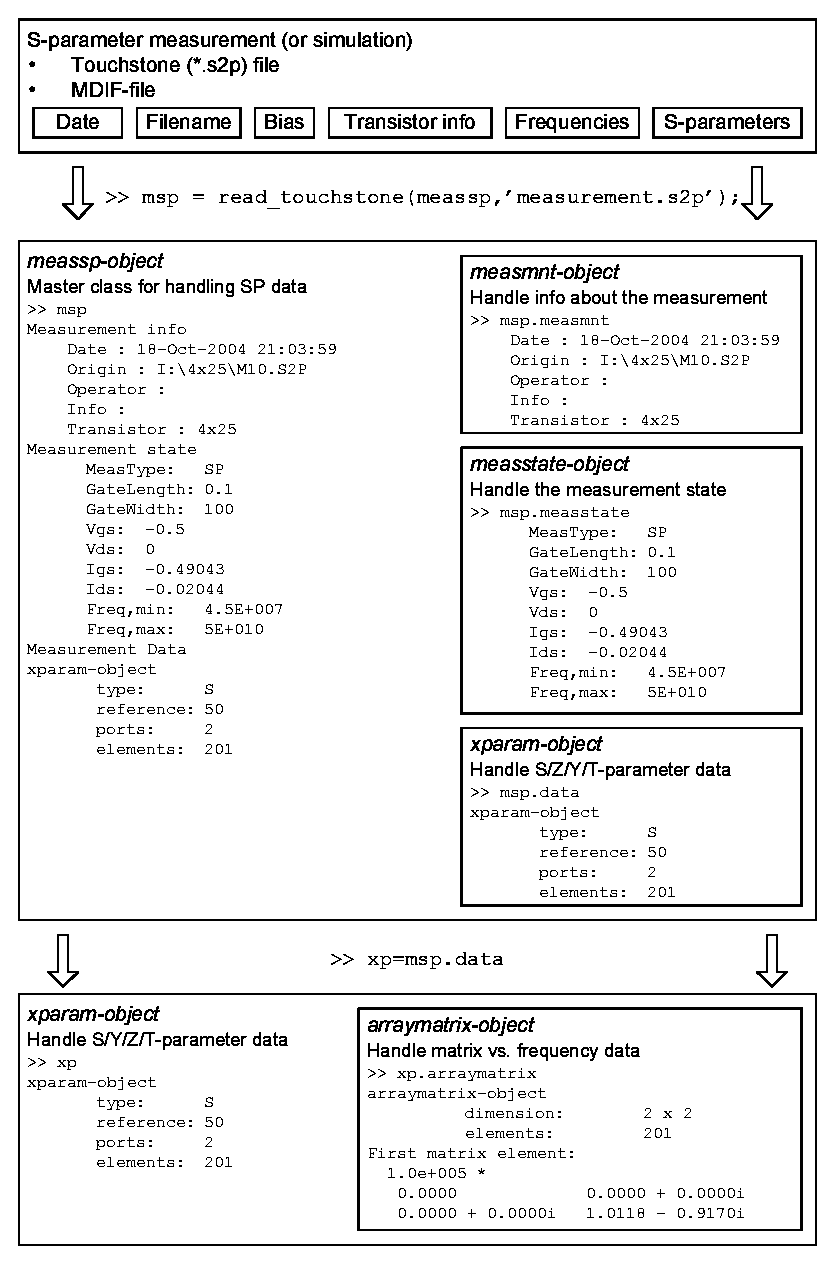
\includegraphics[width=\textwidth]{Figures/ClassOverview3.eps}
  \caption{Overview of the Milou class hierarchy.}\label{fig:ClassHierarchy}
\end{figure}

\subsection{meassp}
\emph{meassp} is the top level class for handling S-parameters.
All functions for reading single measurement files generate
meassp-objects. The resulting measurement information is then
contained its three sub-classes: \emph{measmnt}, \emph{measstate},
and \emph{xparam}.

\subsection{measmnt}
\emph{measmnt} is intended to store information about the
measurement. This can typically include date of measurement, the
measurement operator, the file origin, the transistor type etc.

\subsection{measstate}
\emph{measstate} contains numerical data describing the
measurement conditions. Typically, this is gate bias voltage,
drain current, frequencies, gate width, pulse length, temperature,
etc.

\subsection{xparam}
\emph{xparam} contains the actual S-parameter data. Or, in fact,
it can be data of either S, Y, Z, or T-type. The class keeps track
of which type of data it contains and has built in functionality
to convert between them. Moreover, it stores the reference
impedance so that S-parameters may be converted to other
impedances if required. The numerical complex S/Y/Z/T-data is
stored in an \emph{arraymatrix} object.

\subsection{arraymatrix}
\emph{arraymatrix} is the low level class that is used to
implement matrix multiplication, inversion, conjugate transpose,
addition etc. ``per frequency'', as is needed e.g. for conversion
between Z- and S parameters.

\subsection{Additional classes}
In addition to the classes described above, there exists also a
few other classes that handle sweeps of measurements and
model/netlist generation. These are described later in
\secref{sweeps} and \secref{mna}, respectively.
